\section{Grupos funcionales y jerarquías}

En esta fase, una vez definidos los elementos de datos y funcionales, vamos a
organizarlos agrupándolos en unidades funcionales que nuestras personas el
trabajo en una tarea y la transición entre tareas. Para mostrarlo de manera más
visual hemos realizado un diagrama en árbol, para el que hemos usado el
programa \underline{\href{https://www.drawio.com/}{draw.io}}. Tras un análisis, 
hemos obtenido el resultado que observamos en la figura \ref{fig:jerarquias}, el cuál explicamos a 
continuación:
\begin{figure}[H]
      \centering
      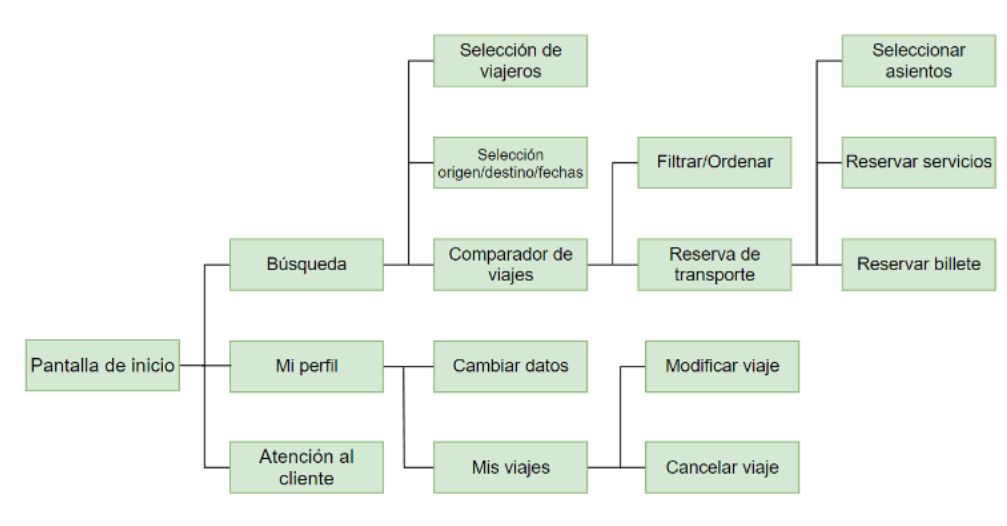
\includegraphics[width=0.8\linewidth]{./Imagenes/jerarquia.png}
      \caption{Diagrama de jerarquías de funciones}
      \label{fig:jerarquias}
\end{figure}

\begin{itemize}
    \item La pantalla de inicio contiene los elementos de búsqueda, atención al cliente y mi perfil.
    \item El elemento de búsqueda es el componente principal por lo que ocupa gran espacio en la interfaz. Al usarla podrás realizar la selección de origen destino y/o fechas, así como de los viajeros. Estas opciones sirven como filtro a la hora de realizar la comparación, que se muestra a continuación.
    \item En el apartado de Comparador de viajes puedes ver todos los que cumplen los criterios anteriormente mencionados. Además puedes cambiar los filtros anteriores y/u ordenarlos según distintos criterios. Además podrás seleccionar si quieres que se muestren solo los viajes accesibles para personas con discapacidad física.
    \item Una vez te interesas por un viaje, pasarás al apartado de Reserva de transporte. Aquí se mostrarán todos los datos de manera clara, como se marcó en los requisitos, además de poder elegir los asientos y realizar la propia reserva del billete.
    \item En el apartado Mi perfil se puede cambiar los datos del usuario (nombre, correo, teléfono, etc) además de poder ver las reservas pasadas, pudiendo tanto cancelar el viaje como modificarlo (fecha u hora, siempre que lo permita la compañía).
    \item Como se comentó en el apartado anterior, se podrá acceder al apartado de atención al cliente desde cualquier punto de la aplicación.
    \item Un principio que podría ser útil para la aplicación es la programación orientada a objetos, debido a que tenemos distintas partes que podrían ser encapsuladas en éstos, como son los viajes.
    \item En cuanto a los patrones, uno de lo que podría usarse sería el patrón Singleton ya que asegura que cada clase tenga una única instancia, controla el acceso a cada recurso y tiene un control estricto de las variables disponibles.
\end{itemize}

\subsection{Orden general en que se usarán los elementos}

\begin{enumerate}

      \item Cambiar la configuración de idioma y moneda.
      \item Acceder a \textit{Atención al cliente} desde la \textit{Página principal}.
      \item Acceder a \textit{Perfil} desde la \textit{Página principal}.
      \item Funcionalidad principal: comparar distintas opciones de transportes según las
            necesidades.

\end{enumerate}

\subsection{Principios y patrones usados}

\begin{itemize}

      \item \textbf{Principio de proximidad.} Al agrupar elementos similares conseguimos que el usuario sepa que están relacionados, facilitando así el aprendizaje. Así como mejorar la memorabilidad, ya que el usuario puede relacionarlos mentalmente y recordarlos como grupo.
            Por ejemplo, la moneda y el idioma se han puesto cerca porque son dos elementos de configuración.
      \item \textbf{Principio de cierre.} Tendemos a buscar un único elemento simple.
            En nuestro caso, hemos puesto una barra deslizante para ver todo el contenido de la página.
      \item \textbf{Principio.} Los elementos de configuración, perfil y ayuda emplean los elementos de otros sistemas para que sea más fácil y rápido.
      \item \textbf{Principio de visibilidad y feedback.} La interfaz emplea distintos mecanismos para transmitir su estado actual y las acciones posibles en un determinado momento.
            Por ejemplo, en la pantalla de Comparador, pone los pasos que quedan para finalizar el proceso.
      \item \textbf{Ley de Von Restorff.} Destacar una funcionalidad por encima del resto.
            En la Página principal, queremos dar más importancia a la barra de búsqueda ya que es el objetivo principal de nuestra aplicación

\end{itemize}
